\chapter{A WaccApp frontend tervezési folyamata}

A WaccApp frontendjének kialakítása nem egyetlen kész felület megvalósításával indult, hanem fokozatos tervezési és fejlesztési folyamat eredménye volt. A projekt kezdetén az elsődleges cél az volt, hogy a WhatsApp Business API-ra épülő üzenetküldés böngészőből is kezelhető legyen. A fejlesztés során azonban egyre világosabbá vált, hogy az egyszerű üzenetküldő űrlap önmagában nem elegendő. A rendszernek sablonos kommunikációt, kérdőíves folyamatokat, médiafájlok kezelését, időzített küldéseket, beszélgetés-visszakövetést, szűrést és egyszerű válaszösszesítést is támogatnia kellett.

A tervezés kiindulópontja az volt, hogy a felhasználó ne technikai végpontokban és API-hívásokban gondolkodjon, hanem érthető kommunikációs műveletekben. A frontendnek ezért köztes értelmező rétegként kellett működnie a felhasználói szándék és a háttérrendszer által elvárt adatszerkezet között. A felhasználó egy címzettet, üzenetet, sablont, kérdőívet, fájlt vagy időpontot ad meg, a frontend pedig ezeket olyan formába rendezi, amely továbbítható a backend felé.

A tervezési folyamat legfontosabb kérdése az volt, hogyan lehet a rendszer eltérő funkcióit úgy elkülöníteni, hogy azok önállóan is áttekinthetők legyenek, de közben egységes alkalmazásként működjenek. A WaccApp nem klasszikus egyoldalas alkalmazásként készült, hanem több HTML-nézetből álló frontendként. Ez a döntés abból következett, hogy a fő funkciók eltérő felhasználói helyzeteket képviselnek. Más felületet igényel egy gyors üzenet elküldése, egy beszélgetés visszanézése, egy kérdőív szerkesztése, egy szűrés lefuttatása vagy egy időzített küldés előkészítése.

\section{A fő felhasználói folyamatok meghatározása}

A frontend tervezésének első lépése a fő felhasználói folyamatok meghatározása volt. A WaccApp nem egyetlen műveletet kezel, ezért a tervezés során külön kellett választani azokat a helyzeteket, amelyekben a felhasználó más céllal használja a rendszert. A legfontosabb folyamatok az üzenetküldéshez, a sablonos kommunikációhoz, a kérdőívkezeléshez, a médiafájlok küldéséhez, az időzített műveletekhez, a beszélgetések visszakövetéséhez és az adatok szűréséhez kapcsolódtak.

Az egyedi üzenetküldés volt a legegyszerűbb felhasználói folyamat. Ebben az esetben a felhasználó megadja a címzettet, kitölti az üzenetszöveget, majd elindítja a küldést. A tervezés célja az volt, hogy ez a folyamat kevés lépésből álljon, ugyanakkor a frontend már a küldés előtt felismerje az alapvető hibákat, például a hiányzó címzettet vagy az üres üzenettartalmat.

A sablonos üzenetküldés ennél kötöttebb folyamatot igényelt. Itt nemcsak címzettet és üzenettartalmat kell kezelni, hanem sablonnevet, nyelvi beállítást és paramétereket is. Emiatt ezt a működést tervezési szinten is el kellett választani az egyszerű szöveges üzenetküldéstől. Ha a két folyamat ugyanabban a merev űrlapban jelent volna meg, a felhasználó számára könnyen bizonytalanná válhatott volna, hogy melyik mező melyik küldési módhoz tartozik.

A kérdőívkezelés külön tervezési figyelmet igényelt, mert itt nem egyszeri küldésről, hanem több lépésből álló kommunikációs logikáról van szó. A felhasználó kérdéseket, válaszlehetőségeket és válaszfüggő folytatásokat állít be. Ezért a kérdőívet nem egyszerű kérdéslistaként kellett kezelni, hanem olyan folyamatmodellként, amelyben egy válasz meghatározhatja a következő lépést.

A kommunikáció visszakövetése szintén önálló felhasználói folyamatként jelent meg. A rendszerben nemcsak az számít, hogy egy üzenet elküldhető-e, hanem az is, hogy később ellenőrizhető legyen, mi történt. A felhasználónak látnia kell az elküldött és beérkezett üzeneteket, valamint egy adott kontakthoz tartozó beszélgetés teljesebb folyamatát. Ez vezetett a lista jellegű nézetek és a chat-szerű beszélgetésnézet elkülönítéséhez.

A szűrés és az egyszerű válaszösszesítés már nem új kommunikációs műveletet indít, hanem a meglévő adatok visszakeresését és alapvető értelmezését támogatja. Itt a tervezés középpontjába a feltételek összeállítása, a név és telefonszám kapcsolatának kezelése, a dátumintervallum értelmezése és az eredmények áttekinthető megjelenítése került.

\section{A nézetekre bontás indoklása}

A fő felhasználói folyamatok meghatározása után a következő tervezési döntés az volt, hogy ezek a folyamatok milyen felületi szerkezetben jelenjenek meg. Elméletileg minden funkció elhelyezhető lett volna egyetlen központi oldalon, ez azonban a WaccApp esetében gyorsan túlzsúfolt és nehezen tanulható felületet eredményezett volna. A rendszerben szereplő feladatok eltérő logikát követnek, ezért indokolt volt a többnézetes felépítés.

Az \path{index.html} központi indítófelületként kapott szerepet, mert innen indulnak a fő küldési műveletek. Ide tartozik az egyedi üzenetküldés, a sablonküldés, a kérdőívindítás, a médiafájl küldése és az időzített küldés. Az \path{index.html} tehát nem egyszerű kezdőoldal, hanem a kommunikációs műveletek előkészítésének és indításának helye.

A kommunikáció visszakövetésére külön nézetek készültek. A \path{messages.html} és a \path{sent-messages.html} a beérkező és elküldött üzenetek listaalapú áttekintését támogatják, míg a \path{conv.html} egy adott kontakthoz kapcsolódó beszélgetést jelenít meg időrendi formában. Ez a felosztás azért volt szükséges, mert más felület kell a gyors listázáshoz, és más akkor, amikor a felhasználó egy teljesebb beszélgetési folyamatot szeretne értelmezni.

A \path{filter.html} önálló nézetként kapott helyet, mert a szűrés nem illeszkedik természetesen az üzenetküldő oldalba. A szűrés során a felhasználó nem új tartalmat hoz létre, hanem korábbi kommunikációs eseményeket keres vissza. Emiatt ezen az oldalon a feltételek megadása, az eredmények megjelenítése és az alapvető összesítés vált elsődlegessé.

A kérdőíves működéshez külön szerkesztőfelületek tartoztak. A \path{questionnaire.html} a szöveges vagy számalapú válaszlogikájú kérdőívekhez kapcsolódik, míg a \path{template.html}, a \path{template-menu.html} és a \path{template-single.html} a sablonos, gombos válaszokra épülő folyamatokat támogatja. Ez a bontás azért volt indokolt, mert a kérdőívszerkesztés nem pusztán adatbevitel, hanem kérdések, válaszok és következő lépések közötti kapcsolatok kezelése.

A nézetekre bontás így egyszerre szolgált használhatósági és fejlesztői célt. A felhasználó számára minden oldal egy jól felismerhető feladat köré épül, fejlesztői oldalról pedig könnyebbé válik a funkciók elkülönítése, javítása és későbbi bővítése.

\section{A tervezett adatáramlás}

A WaccApp frontendjének tervezésekor fontos szempont volt, hogy a különböző nézetek eltérő feladatokat látnak el, mégis hasonló adatáramlási logikára épüljenek. A legtöbb folyamat a felhasználói bevitellel indul, ezt kliensoldali ellenőrzés követi, majd API-hívás történik, végül a válasz alapján frissül a felület.

Az üzenetküldés adatáramlása az \path{index.html} oldalon kezdődik. A felhasználó megadja a címzettet és az üzenet tartalmát, a JavaScript összegyűjti az adatokat, ellenőrzi a kötelező mezőket, majd a megfelelő végpont felé továbbítja a kérést. A válasz alapján a frontend sikeres vagy hibás állapotot jelenít meg. Ez az alapfolyamat adta a többi küldési típus tervezési mintáját is.

Sablonos küldés esetén az adatáramlás kiegészül a sablon nevével, a nyelvi beállítással és a paraméterekkel. A frontendnek ebben az esetben nemcsak azt kell ellenőriznie, hogy van-e címzett, hanem azt is, hogy a sablonhoz szükséges adatok rendelkezésre állnak-e. Ez azért fontos, mert egy hiányos sablonkérés később szerveroldali vagy platformszintű hibát okozhatna.

A kérdőívek adatáramlása összetettebb, mert a felhasználó nem egyetlen üzenetet állít össze, hanem egy kommunikációs folyamat szerkezetét. A \path{questionnaire.html} esetében a kérdések, válaszok és következő lépések olyan adatszerkezetté állnak össze, amely később menthető és indítható. A \path{template.html} ugyanezt a gondolkodást a sablonos, gombos válaszlogikához igazítja.

A \path{conv.html} adatáramlása lekérdezésalapú. A nézet egy adott kontakthoz tartozó korábbi üzeneteket kér le, majd azokat időrendi beszélgetésként jeleníti meg. A frontend feladata itt az, hogy a nyers üzenetadatokat ne technikai rekordként mutassa meg, hanem felhasználói szempontból értelmezhető kommunikációs folyamatként.

A \path{filter.html} esetében az adatáramlás a szűrési feltételekből indul. A felhasználó megadja a keresési szempontokat, a frontend ezekből lekérdezési paramétereket állít össze, majd az API-választ eredménylistaként vagy alapvető összesítésként jeleníti meg. Ennél a folyamatnál különösen fontos volt, hogy az üres találat ne legyen félreérthető. A felhasználónak tudnia kell, hogy a keresés lefutott, csak nem adott eredményt.

Az adatáramlási logika szemléltetésére az egyedi üzenetküldés folyamata használható a legátláthatóbb példaként. Ez a folyamat azért alkalmas modellként, mert ugyanazokat az alaplépéseket tartalmazza, amelyek a WaccApp több más műveletében is megjelennek: a felhasználói adatbevitel után kliensoldali ellenőrzés történik, majd a frontend API-kérést indít, végül a válasz alapján frissíti a felület állapotát.

\begin{figure}[H]
    \centering
    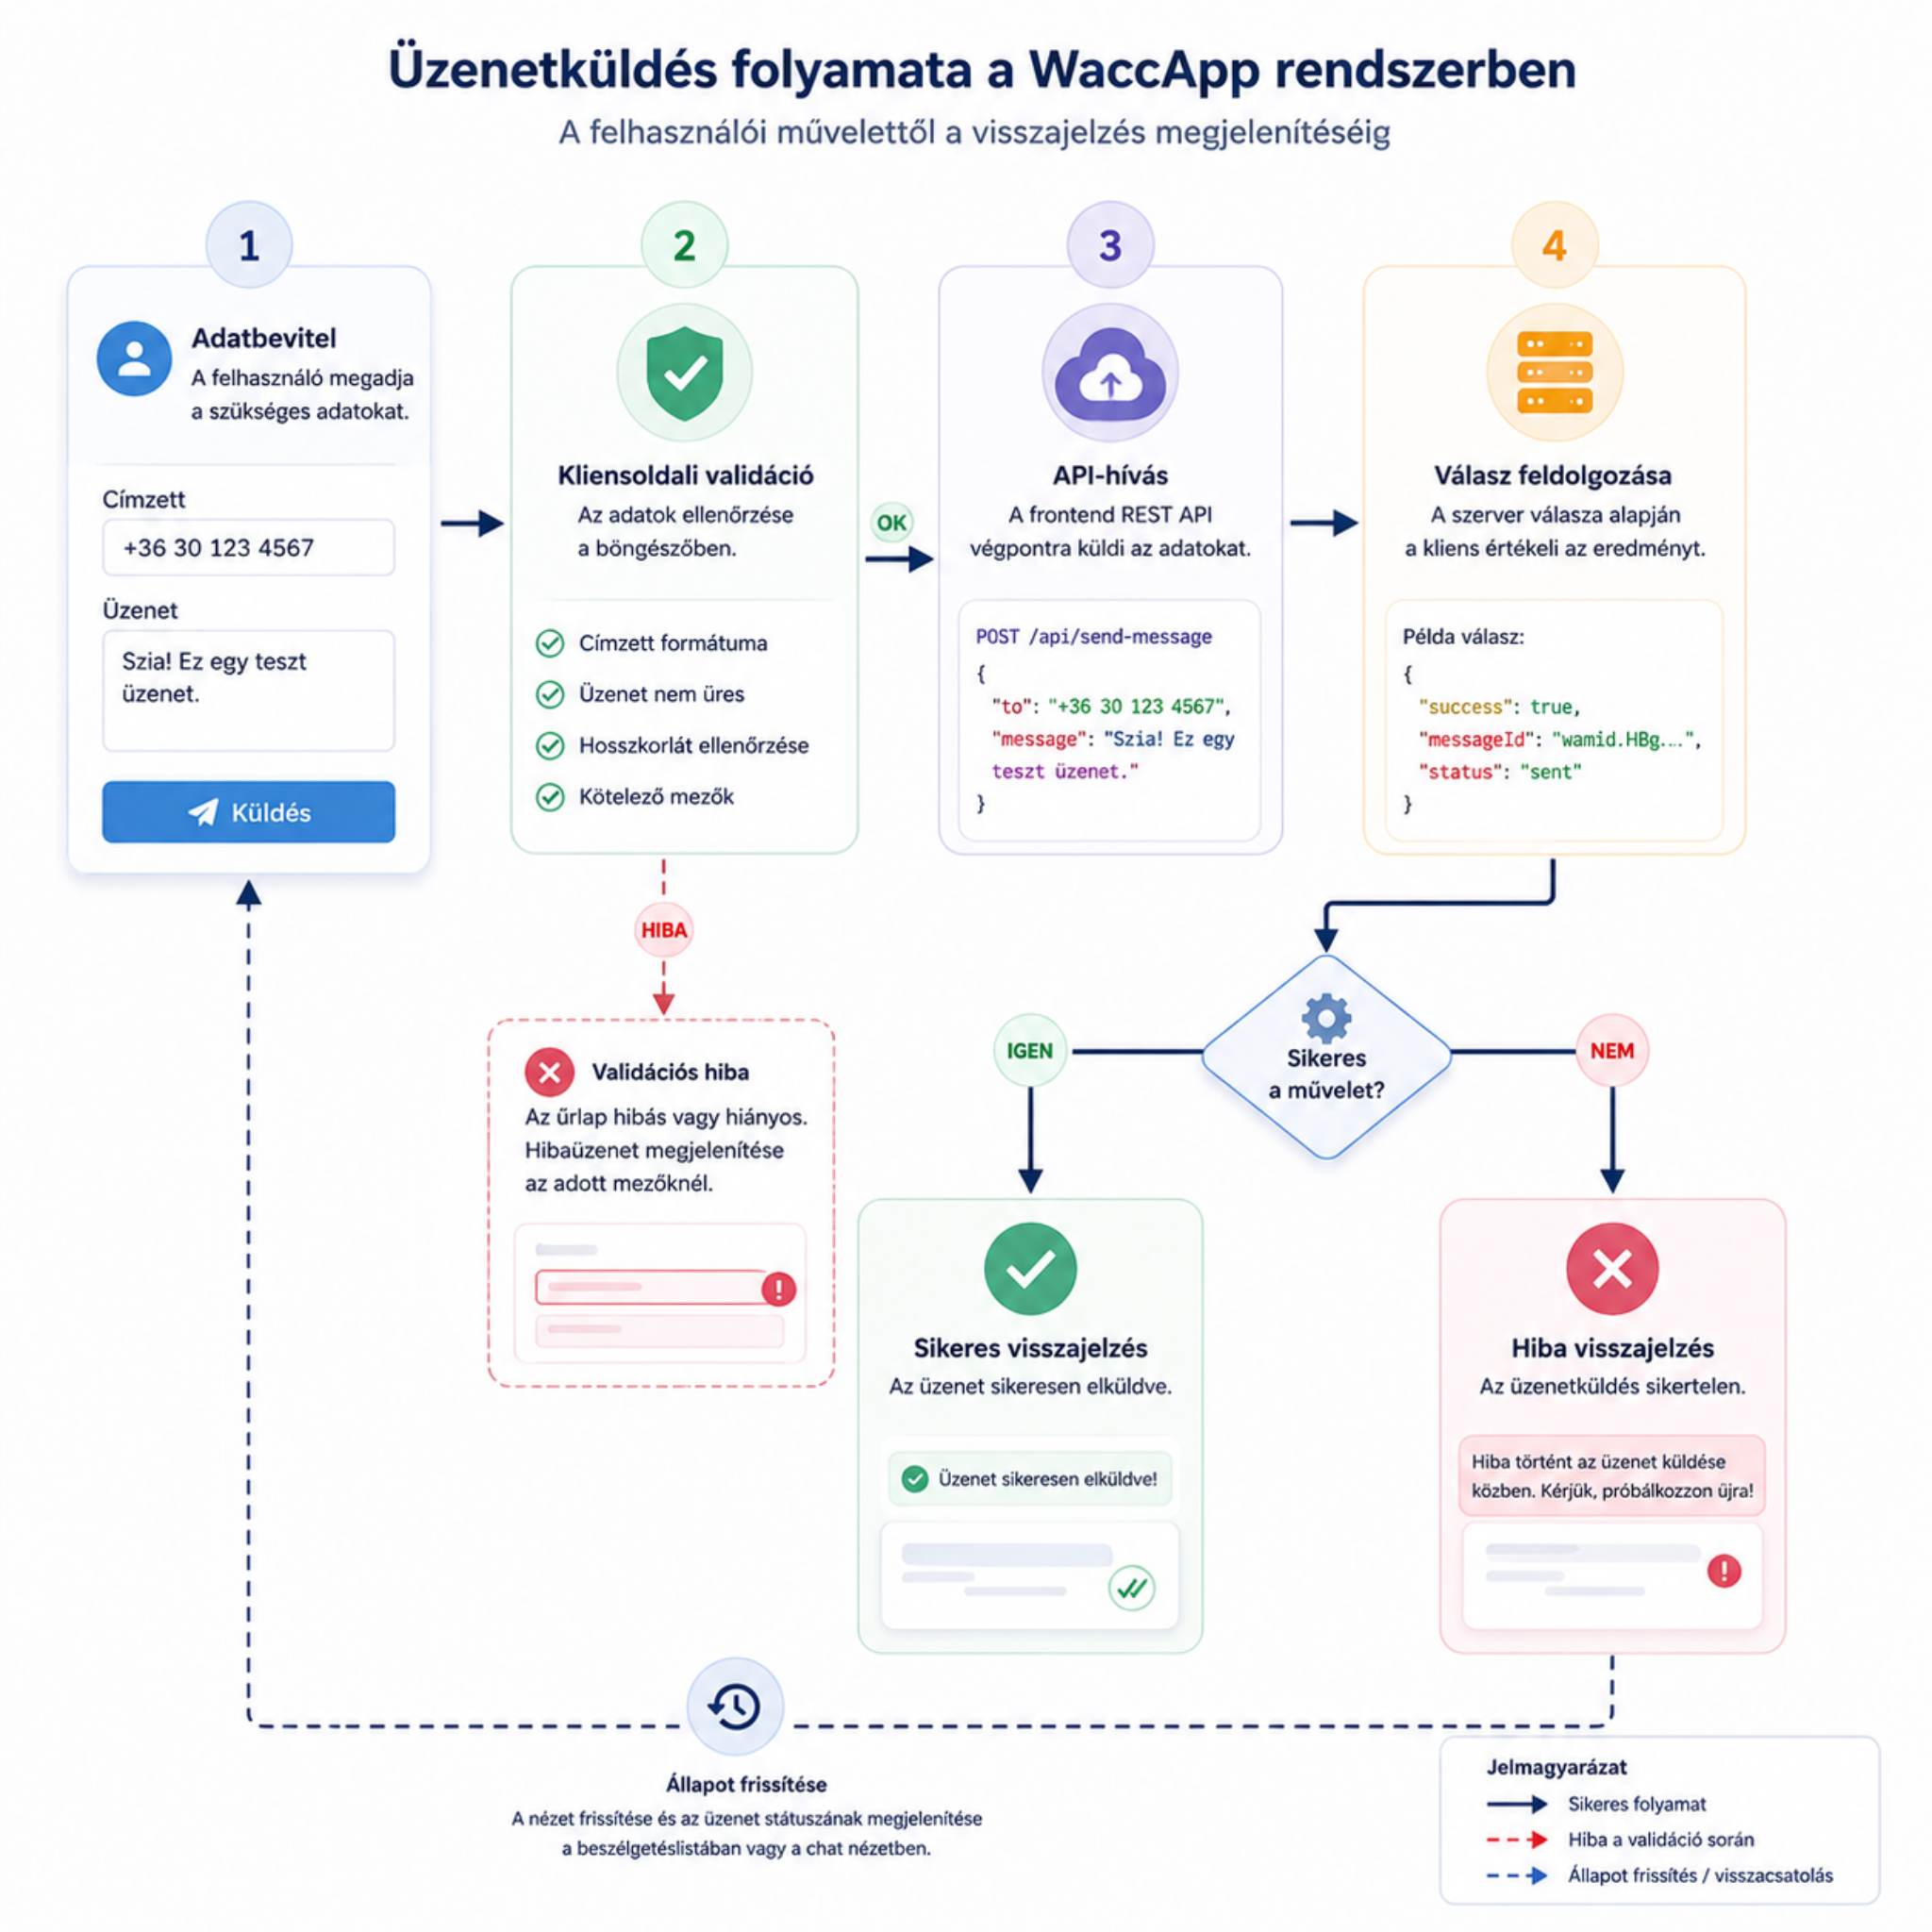
\includegraphics[width=0.92\textwidth]{images/waccapp-uezenetkuldes-folyamata.png}
    \caption{Az üzenetküldés tervezett frontendfolyamata a WaccApp rendszerben.}
    \label{fig:uzenetkuldes-folyamata}
\end{figure}

Az adatáramlási logikát az \ref{fig:uzenetkuldes-folyamata}. ábra szemlélteti. Az ábra a frontend szempontjából fontos folyamatot mutatja be, vagyis azt, amit a felhasználó közvetlenül érzékel. A validációs ág azért szerepel külön, mert hibás vagy hiányos adat esetén a kérésnek nem célszerű eljutnia a szerveroldali feldolgozásig. Sikeres válasz esetén a felület visszajelzést ad, hiba esetén pedig javítható állapotot jelenít meg. Ez a folyamat később a sablonos küldésnél, a médiaküldésnél és az időzített műveleteknél is hasonló alaplogikára épül, csak az adatcsomag és az ellenőrzések köre bővül.

\section{Validációs és hibakezelési tervezés}

A validáció tervezésekor abból kellett kiindulni, hogy a WaccApp több olyan műveletet kezel, ahol egy hiányzó vagy hibás adat a teljes kommunikáció sikertelenségét okozhatja. A validáció célja ezért nem pusztán formai ellenőrzés volt, hanem a nyilvánvalóan hibás kérések megelőzése.

Az \path{index.html} esetében a validáció első szintje a kötelező mezők ellenőrzése. Egyedi üzenetküldésnél szükséges a címzett és az üzenetszöveg. Sablonos küldésnél ellenőrizni kell a sablon kiválasztását és a paramétereket. Médiafájl küldésekor vizsgálni kell, hogy a felhasználó választott-e fájlt. Időzített küldésnél pedig az időpont értelmezhetősége is fontos, mert egy hibás időpont később sikertelen művelethez vezethet.

A kérdőívszerkesztő nézeteknél a validáció nemcsak mezőszintű, hanem logikai jellegű is. Itt nem elegendő azt ellenőrizni, hogy egy kérdés vagy válaszmező ki van-e töltve. Azt is figyelni kell, hogy a válaszokhoz tartozik-e következő kérdés vagy lezárás. Ha ez hiányzik, akkor a kérdőív futás közben megszakadhat.

A \path{filter.html} validációja az értelmezhető keresési feltételeket védi. A dátumintervallum esetében például ellenőrizni kell, hogy a kezdődátum ne legyen későbbi, mint a záródátum. A név és telefonszám kapcsolatánál pedig arra kell figyelni, hogy a felhasználó ne hozzon létre félrevezető párosítást. Egy hibás szűrés nem feltétlenül okoz technikai hibát, de rossz következtetéshez vezethet.

A hibakezelés tervezésénél alapelv volt, hogy a hibaüzenet ne csak megállítsa a folyamatot, hanem segítse a javítást. A felhasználó számára hasznosabb, ha a felület konkrétan jelzi, hogy hiányzik a címzett, üres az üzenetszöveg, nincs kiválasztott fájl, hibás az időpont vagy hiányos a kérdőív egyik kapcsolata. Így a felhasználó nem találgat, hanem célzottan tudja javítani az adatot.

Fontos tervezési szempont volt az is, hogy a frontend és a backend felelőssége elkülönüljön. A frontend képes felismerni a hiányzó mezőket és bizonyos formai hibákat, de nem döntheti el véglegesen, hogy egy telefonszám valóban elérhető-e WhatsAppon, vagy hogy a külső platform elfogadja-e az adott műveletet. A kliensoldal feladata ezért az előszűrés és a szerverválaszok érthető megjelenítése.

\section{Állapotkezelési tervezés}

A WaccApp több művelete aszinkron módon működik, ezért a frontend tervezésekor külön figyelmet kellett fordítani az állapotkezelésre. Egy üzenetküldés, fájlfeltöltés, szűrés, beszélgetésbetöltés vagy kérdőívmentés nem mindig ad azonnali eredményt. A felhasználónak mégis érzékelnie kell, hogy a művelet elindult, folyamatban van, sikeresen lezárult vagy hibára futott.

A tervezett állapotmodell négy alaphelyzetre épült. Nyugalmi állapotban a felület használatra kész. Feldolgozás alatti állapotban a kérés már elindult, de az eredmény még nem ismert. Sikeres állapotban a rendszer visszajelzi, hogy a művelet rendben lezárult. Hibás állapotban pedig a felület jelzi, hogy a folyamat nem sikerült, és lehetőség szerint megmutatja a hiba okát is.

Az \path{index.html} esetében ez főként a küldési műveleteknél fontos. Ha a felhasználó elküld egy üzenetet, sablont vagy médiafájlt, a felületnek jeleznie kell, hogy a rendszer feldolgozza a kérést. Enélkül a felhasználó könnyen újra megnyomhatja a gombot, vagy azt hiheti, hogy a rendszer nem reagált.

A \path{filter.html} esetében az állapotkezelés az adatbetöltés és az eredmények értelmezése miatt lényeges. A keresés eredménye lehet találati lista, de lehet üres eredmény is. A kettő között felhasználói szempontból fontos különbség van: az üres eredmény nem ugyanaz, mint a sikertelen lekérdezés.

A \path{conv.html} beszélgetésnézetben az állapotkezelés célja az, hogy a beszélgetés betöltése ne tűnjön bizonytalannak. Ha nincs megjeleníthető kommunikációs előzmény, azt másként kell kezelni, mint amikor az adatok betöltése hibára futott. Ez segít abban, hogy a felhasználó ne rendszerhibaként értelmezzen egy üres beszélgetést.

Az időzített küldéseknél az állapotkezelés kiterjedtebb, mert a művelet rögzítése és tényleges végrehajtása időben elválik egymástól. A felhasználónak először azt kell látnia, hogy az ütemezés mentése sikerült-e, később pedig azt, hogy a művelet várakozó, sikeres vagy sikertelen állapotban van-e. Emiatt az időzítés nem egyszerű dátummezőként, hanem állapotokkal rendelkező kommunikációs folyamatként jelent meg a tervezésben.

\section{A tervezési folyamat összegzése}

A WaccApp frontendjének tervezése során a legfontosabb cél az volt, hogy a WhatsApp Business API-ra épülő összetett kommunikációs működés a felhasználó számára kezelhető webes folyamatokká alakuljon. A tervezés nemcsak a felület vizuális kialakításáról szólt, hanem a fő felhasználói folyamatok, a nézetek felelőssége, az adatáramlás, a validáció, a hibakezelés és az állapotjelzések meghatározásáról is.

A többnézetes frontend kialakítása azért bizonyult megfelelő döntésnek, mert a rendszer fő funkciói eltérő felhasználói helyzeteket képviselnek. Az \path{index.html} a küldési műveletekre, a \path{conv.html} a beszélgetések megjelenítésére, a \path{filter.html} a visszakeresésre, a \path{questionnaire.html} és a \path{template.html} pedig a kérdőíves és sablonos folyamatokra koncentrál. Ez a bontás egyszerre teszi átláthatóbbá a használatot és könnyebben karbantarthatóvá a fejlesztést.

A tervezési folyamat másik fontos eredménye az egységes működési minta kialakítása volt. A fő folyamatok eltérő célt szolgálnak, de alaplogikájuk hasonló: a felhasználó adatot ad meg, a frontend ellenőriz, API-kérést indít, majd a válasz alapján frissíti a felületet. Ez az ismétlődő minta biztosítja, hogy a WaccApp több HTML-nézetből állva is egységes frontendként működjön.
